\documentclass[a4paper,12pt]{report}

% --- REQUIRED PACKAGES ---
\usepackage[utf8]{inputenc}
\usepackage[T1]{fontenc}
\usepackage[english]{babel}
\usepackage{graphicx}
\usepackage{hyperref}
\usepackage{booktabs}
\usepackage{geometry}
\usepackage{setspace}
\usepackage{titlesec}
\usepackage{amsmath}
\usepackage{amssymb}
\usepackage{listings}
\usepackage{xcolor}
\usepackage{fancyhdr}
\usepackage{tocloft}
\usepackage{mathptmx} % Chinh font chu Times New Roman chuan bao cao khoa hoc / luan van

% --- GEOMETRY & SPACING ---
\geometry{
    a4paper,
    left=35mm,
    right=20mm,
    top=30mm,
    bottom=30mm,
}
\setstretch{1.5} % Dan dong 1.5 tao khoang cach chuan de doc va dat do dai tieu chuan

% --- CODES LISTING STYLE ---
\definecolor{codegreen}{rgb}{0,0.6,0}
\definecolor{codegray}{rgb}{0.5,0.5,0.5}
\definecolor{codepurple}{rgb}{0.58,0,0.82}
\definecolor{backcolour}{rgb}{0.96,0.96,0.94}

\lstdefinestyle{pythonstyle}{
    backgroundcolor=\color{backcolour},   
    commentstyle=\color{codegreen},
    keywordstyle=\color{blue}\bfseries,
    numberstyle=\tiny\color{codegray},
    stringstyle=\color{codepurple},
    basicstyle=\ttfamily\footnotesize,
    breakatwhitespace=false,         
    breaklines=true,                 
    captionpos=b,                    
    keepspaces=true,                 
    numbers=left,                    
    numbersep=5pt,                  
    showspaces=false,                
    showstringspaces=false,
    showtabs=false,                  
    tabsize=4
}
\lstset{style=pythonstyle}

% --- HEADER AND FOOTER ---
\pagestyle{fancy}
\fancyhf{}
\fancyhead[R]{\thepage}
\fancyhead[L]{\leftmark}
\renewcommand{\headrulewidth}{0.5pt}

% --- DOCUMENT ---
\begin{document}

% =========================================================
% COVER PAGE
% =========================================================
\begin{titlepage}
    \centering
    \begin{singlespace}
        \large \textbf{UNIVERSITY OF SCIENCE AND TECHNOLOGY OF HANOI} \\
        \large \textbf{DEPARTMENT OF INFORMATION AND COMMUNICATION TECHNOLOGY} \\
        \vspace{1.5cm}
        \includegraphics[width=0.45\textwidth]{usth_logo} % Logo truong
        \vspace{1.5cm}
        
        \LARGE \textbf{GRADUATION THESIS REPORT} \\
        \vspace{0.8cm}
        \Huge \textbf{AI Video Assistant: An Automated Video Production Pipeline Using Fine-Tuned Qwen3-TTS and Semantic Vector Search} \\
        \vspace{2.5cm}
        
        \large \textbf{Specialty:} Information and Communication Technology \\
        \large \textbf{Academic Year:} 2025 - 2026
        \vspace{2.5cm}
        
        \begin{flushleft}
            \large
            \textbf{Student Name:} Nguyễn Đăng Vĩ Anh \\
            \textbf{Student ID:} 22BA13017 \\
            \textbf{Supervisor:} ThS. [Tên Giáo Viên Hướng Dẫn] \\
            \textbf{Co-Supervisor:} [Tên Người Đồng Hướng Dẫn - Nếu Có]
        \end{flushleft}
        \vfill
        \large Hanoi, \today
    \end{singlespace}
\end{titlepage}

\newpage

% =========================================================
% ACKNOWLEDGEMENTS
% =========================================================
\chapter*{Acknowledgements}
\addcontentsline{toc}{chapter}{Acknowledgements}
First and foremost, I would like to express my sincere gratitude to my supervisor, ThS. [Tên Giáo Viên Hướng Dẫn], whose constant advice, constructive feedback, and technical support have been invaluable throughout my graduation internship and the writing of this thesis. 

I also wish to thank all the lecturers and staff of the Department of Information and Communication Technology at the University of Science and Technology of Hanoi (USTH) for providing a competitive yet supportive academic environment, equipping me with the essential skills and knowledge required for this research.

Lastly, I want to thank my family, peers, and friends who have offered moral support and encouragement during the intensive phases of development, GPU training runs on cloud nodes, and thesis writing.
\newpage

% =========================================================
% ABSTRACT
% =========================================================
\chapter*{Abstract}
\addcontentsline{toc}{chapter}{Abstract}
In the contemporary digital era, short-form and long-form video content creation on platforms such as YouTube, TikTok, and Facebook Reels has surged. However, the traditional workflow of video editing remains highly manual and repetitive, requiring significant human hours to split scripts, record natural voices, search for relevant context images, and assemble assets onto a timeline. This research designs, implements, and evaluates an \textbf{AI Video Assistant} prototype that automatically converts raw text scripts into finished video timelines for the professional suite DaVinci Resolve.

The proposed pipeline is structured into six functional modules: a text preprocessor for sentence-level segment chunking, a script analyzer using a Large Language Model (Qwen2.5-7B-Instruct) to generate structural metadata, a customized \textbf{Qwen3-TTS} model (1.7B parameters) fine-tuned on personalized voice samples for natural speech synthesis, an AI image retrieval engine utilizing \textbf{CLIP} embeddings and \textbf{FAISS} vector search for semantic matching, a timeline duration parser, and an exporter generating \textbf{Final Cut Pro XML (FCPXML)} documents. 

For model evaluation, we developed an automated benchmarking suite using the offline \textbf{Faster-Whisper (small)} ASR model to compute the Word Error Rate (WER) against a gold-standard test manifest. The fine-tuned Qwen3-TTS model achieved an average WER of \textbf{15.75\%}, showing highly natural and clear speech synthesis. Furthermore, the FCPXML export enables free DaVinci Resolve users to import the assets directly with automatic alignment, bypassing expensive API calls or Studio licenses.
\newpage

% =========================================================
% LISTS
% =========================================================
\tableofcontents
\newpage
\listoffigures
\newpage
\listoftables
\newpage

% =========================================================
% CHAPTER 1: INTRODUCTION
% =========================================================
\chapter{Introduction}
\label{ch:intro}
\section{Background and Motivation}
In the contemporary global digital landscape, multimedia communication has emerged as the dominant paradigm for knowledge dissemination, public education, corporate marketing, and entertainment. With the meteoric rise of social media platforms specialized in both short-form and long-form video content—such as TikTok, YouTube Shorts, and Facebook Reels—billions of users consume video material daily. This massive, unprecedented consumption rate has created intense pressure on independent content creators, digital marketing agencies, educational institutions, and news organizations. To remain competitive and visible within search algorithms, creators must produce high-quality video drafts within extremely compressed production windows.

However, the post-production editing workflow remains a highly manual, labor-intensive, and repetitive bottleneck. Despite major advancements in digital audio-visual editing workstations (DAWs), a typical editor must still execute a sequential and time-consuming set of tasks:
\begin{enumerate}
    \item \textbf{Script Normalization and Parsing:} The editor must clean raw text scripts, resolve abbreviations, normalize numerical figures, and manually slice the text into logical sentences or paragraphs that represent individual narration blocks.
    \item \textbf{Narration and Speech Sourcing:} The editor must record high-quality voiceovers using physical recording setups (microphones, sound isolation) or deploy commercial Text-to-Speech (TTS) engines. Unfortunately, standard TTS outputs sound robotic, flat, and fail to capture natural human prosody, localized Vietnamese tones, or emotional variations, leading to low audience retention.
    \item \textbf{B-roll Visual Asset Sourcing:} The editor must search through extensive stock database collections or local file directories to find image files and video clips that match the semantic context of each narration block. This search is traditionally limited to exact-match text keywords or tags, which is highly ineffective when assets are named arbitrarily (e.g., raw camera exports).
    \item \textbf{Timeline Assembly and Synchronization:} The editor must import the media files into a timeline, manually place each audio clip onto its track, and stretch or trim the corresponding visual asset frame-by-frame to match the exact start and end times of the narration. This timeline alignment step is extremely tedious and is prone to synchronization errors or visual drift.
\end{enumerate}

To alleviate this post-production bottleneck, recent breakthroughs in Generative Artificial Intelligence (AI) present a viable path toward complete automation. Modern Large Language Models (LLMs) like the Qwen2.5 series excel at structural prompt processing and semantic script segmentation. In parallel, neural speech synthesis has shifted from multi-stage models (such as Tacotron2 generating Mel-spectrograms followed by vocoders) to single-stage autoregressive architectures like Qwen3-TTS. These models process speech using quantized neural audio codec tokens, capturing natural human voice characteristics, breath patterns, and emotional cues. Additionally, cross-modal neural networks like Contrastive Language-Image Pre-training (CLIP) combined with dense vector database search libraries like FAISS enable real-time semantic retrieval of visual assets without relying on manual tag metadata.

By combining these AI components into a unified, modular Python-based pipeline, the tedious aspects of initial draft video creation can be completely automated. This graduation project focuses on the design, implementation, and evaluation of an \textbf{AI Video Assistant} prototype. The system processes raw Vietnamese scripts and local asset directories, automatically performs voice cloning and semantic visual retrieval, and outputs a synchronized timeline document that can be imported directly into professional editors like DaVinci Resolve, establishing a seamless, file-based post-production workflow.
\section{Problem Statement}
Given a raw, unstructured Vietnamese narration script $T_{\text{script}}$ and a local directory containing a set of visual B-roll assets $I_{\text{assets}} = \{i_1, i_2, \dots, i_K\}$, the objective of the system is to construct a synchronized, timing-aligned video timeline serialized as a Final Cut Pro XML (FCPXML v1.5) document $M_{\text{timeline}}$. This mapping is mathematically expressed as:
\begin{equation}
    M_{\text{timeline}} = f(T_{\text{script}}, I_{\text{assets}}; \theta_{\text{TTS}}, \theta_{\text{CLIP}})
\end{equation}
where $\theta_{\text{TTS}}$ represents the parameters of the fine-tuned, personalized text-to-speech (TTS) model and $\theta_{\text{CLIP}}$ represents the parameters of the cross-modal embedding model. The mapping function $f$ must ensure that every visual slide $v_m$ matches the exact duration of the spoken narration of its corresponding script segment $p_m$.

The system operates on two primary inputs: the Vietnamese narration script ($T_{\text{script}}$), which is a raw text containing noise, punctuation, and abbreviations (e.g., ``ThS.'', ``TS.'') requiring normalization and sentence-level segmentation, and a database of visual assets ($I_{\text{assets}}$) consisting of image files under unstructured names (e.g., ``IMG\_1002.jpg'') without tag metadata. The terminal output is the FCPXML timeline $M_{\text{timeline}}$, which maps the synthesized voice clips sequentially to audio track A1 and the selected B-roll images to video track V1, aligning their frame-accurate start and end points ($S_m, E_m$) based on the project framerate.

To resolve this mapping theoretically, the pipeline must overcome four core technical barriers. First, the linguistic normalization and pacing barrier requires parsing script text while avoiding false splits on abbreviations and grouping sentences to limit visual pacing (e.g., at most two sentences per slide). Second, the personalized speech synthesis barrier requires fine-tuning a 1.7B parameter autoregressive model (Qwen3-TTS) under local VRAM constraints to clone the user's voice naturally. Third, the cross-modal semantic retrieval barrier requires encoding both images and segment text into a shared vector space using CLIP embeddings and FAISS indices to perform similarity searches based on semantic context rather than filenames. Lastly, the professional editor integration barrier requires generating compliant FCPXML v1.5 files to bypass paid license scripting API constraints, ensuring a seamless timeline setup.
\newpage

\section{Research Objectives}
To address the challenges of repetitive manual video editing, unnatural voice synthesis, visual matching limitations, and professional software automation barriers, this project pursues five core research objectives:
\begin{enumerate}
    \item \textbf{Design a Vietnamese Script Parser:} Implement a modular preprocessing and tokenizing pipeline to normalize Vietnamese text inputs (handling carriage returns, whitespaces, and punctuation), identify sentence boundaries, and segment them based on visual pacing constraints to ensure a dynamic clip duration.
    \item \textbf{Train a Custom Text-to-Speech Model:} Fine-tune a 1.7 Billion parameter autoregressive Qwen3-TTS model using Supervised Fine-Tuning (SFT) on clean, personal voice recordings to clone the user's specific voice, capturing emotional prosody, breath pauses, and natural speech patterns.
    \item \textbf{Implement a Semantic B-roll Retrieval Engine:} Build an offline image search index utilizing pre-trained CLIP embeddings and a FAISS vector database. The engine must project images and text prompts into a shared 512-dimensional vector space to execute real-time, context-matching lookups.
    \item \textbf{Develop an FCPXML Timeline Exporter:} Program a metadata parser to compute audio durations, map them to exact frame boundaries based on target project frame rates, and compile the layout into Final Cut Pro XML (FCPXML v1.5) documents for direct import.
    \item \textbf{Build an Automatic Evaluation Pipeline:} Develop a local benchmarking suite utilizing the Faster-Whisper ASR model and the Jiwer library to compute the Word Error Rate (WER) of the synthesized audio, providing quantitative validation of voice intelligibility.
\end{enumerate}

\section{Scope of the Project}
The operational boundaries, hardware constraints, and software parameters of this research are defined as follows:
\begin{itemize}
    \item \textbf{Linguistic Range and Script Constraints:} The front-end parser and back-end speech synthesis are optimized specifically for Vietnamese language processing. It is designed to handle standard Vietnamese scripts and does not include an automated text normalizer for multi-lingual code-switching or code-mixing terms.
    \item \textbf{Database Size and Sourcing:} The semantic visual matching is executed over offline local directories of images (such as Flickr8k or custom graphic folders). It does not include active, real-time web crawlers or online API-based stock video searches.
    \item \textbf{Autoregressive Model Scale:} The voice cloning module focuses on Alibaba's Qwen3-TTS 1.7B parameter transformer architecture. SFT training is performed in a hybrid environment (cloud platform training with dual Tesla T4 GPUs and local offline client PC inference).
    \item \textbf{Timeline Target Integration:} Timeline generation targets the FCPXML v1.5 standard, specifically optimized for DaVinci Resolve. It is compatible with both the free and Studio editions of DaVinci Resolve and operates as a file-based import script rather than active, running TCP socket scripting.
\end{itemize}

\section{Contributions}
This thesis contributes a modular, reproducible software framework that automates the transition from a text script to a synchronized video editing layout. The specific theoretical and engineering contributions are:
\begin{itemize}
    \item \textbf{Custom Personalized Offline Voice Synthesis:} Successful supervised fine-tuning (SFT) of a 1.7B parameter Qwen3-TTS model on personalized Vietnamese voice recordings, delivering clear, natural voiceovers with emotional prosody.
    \item \textbf{Semantic Vector Search Integration:} Implementation of an offline semantic retrieval system combining CLIP image-text embeddings with a FAISS vector index, enabling microsecond B-roll retrieval based on query context instead of manual file naming.
    \item \textbf{License-Independent Workspace Automation:} A file-based FCPXML timeline builder that calculates wave audio durations, maps them to frame integers, and compiles multi-track import files, allowing free DaVinci Resolve users to bypass paid licensing scripting APIs.
    \item \textbf{Automated Offline Quality Verification Suite:} An end-to-end evaluation pipeline that uses the Faster-Whisper (small) ASR model and Jiwer library to compute the Word Error Rate (WER) of synthesized voiceovers, establishing a systematic method for testing voice model clarity.
\end{itemize}

\section{Thesis Structure}
The remainder of this thesis is organized into seven chapters:
\begin{itemize}
    \item \textbf{Chapter 2 (Background and Related Work)} reviews the theoretical foundations of Transformers, Large Language Models, neural speech models, vector embeddings, and FCPXML structures.
    \item \textbf{Chapter 3 (System Design and Methodology)} details the architecture of the six core pipeline modules and the sequence of data transfers.
    \item \textbf{Chapter 4 (Implementation)} presents the local and cloud hardware configuration, python libraries, and core source code files.
    \item \textbf{Chapter 5 (Evaluation and Results)} reports the quantitative WER scores, qualitative speech errors, and timeline synchronization outcomes.
    \item \textbf{Chapter 6 (Discussion)} discusses research findings, limitations (including the lack of text normalization for code-switching), and how FCPXML solves Studio licensing API limits.
    \item \textbf{Chapter 7 (Conclusion and Future Work)} summarizes the project's outcomes and suggests future work, such as a web interface and video B-roll retrieval.
\end{itemize}
\newpage

% =========================================================
% CHAPTER 2: BACKGROUND AND RELATED WORK
% =========================================================
\chapter{Background and Related Work}
\label{ch:background}

\section{Large Language Models}
Large Language Models (LLMs) represent a significant milestone in natural language processing (NLP), shifting the field from task-specific heuristic models to unified, general-purpose learners. Based on the Transformer architecture, these models leverage the self-attention mechanism to model long-range context dependencies in text:
\begin{equation}
    Attention(Q, K, V) = \text{softmax}\left(\frac{QK^T}{\sqrt{d_k}}\right)V
\end{equation}
where $Q \in \mathbb{R}^{T_q \times d_k}$, $K \in \mathbb{R}^{T_k \times d_k}$, and $V \in \mathbb{R}^{T_k \times d_v}$ represent the query, key, and value matrices projected from token embeddings, and $d_k$ is the scaling factor denoting the dimensionality of the keys. The dot product $QK^T$ measures the raw pairwise similarity between all input tokens. Dividing by the scaling factor $\sqrt{d_k}$ prevents the dot product values from growing extremely large in high dimensions, which would push the softmax function into regions with dangerously small gradients. The softmax activation normalizes these scores into a probability distribution representing attention weights, which are then multiplied by the value matrix $V$ to compute the final context-aware token representation.

To allow the model to attend to information from different representation subspaces simultaneously, modern architectures utilize Multi-Head Attention (MHA):
\begin{equation}
    MultiHead(Q, K, V) = Concat(head_1, head_2, \dots, head_h)W^O
\end{equation}
where each head is calculated as $head_i = Attention(QW_i^Q, KW_i^K, VW_i^V)$ using distinct, learnable weight projection matrices. In this project, the Qwen2.5-Instruct series (ranging from 7B to 14B parameter configurations) is studied. By applying instruction tuning using Supervised Fine-Tuning (SFT) and Reinforcement Learning from Human Feedback (RLHF), these models are optimized to execute complex reasoning, normalize text layouts, and produce structured JSON payloads containing keywords, emotional tones, and visual prompts from raw Vietnamese narration scripts.

\section{Retrieval-Augmented Generation}
Retrieval-Augmented Generation (RAG) is a framework designed to ground Large Language Models on external, verifiable knowledge repositories. LLMs are prone to hallucinating facts due to their lossy parametric memory, which cannot store every detail and becomes outdated quickly. RAG addresses this limitation by dividing the question-answering workflow into three steps: indexing, retrieval, and generation. During indexing, external text documents are parsed, converted into vector representations using embedding models, and stored in a vector index database. When a user submits a query, the retrieval component finds the most semantically relevant document vectors. These documents are converted back to text and appended to the model's prompt context, allowing the LLM to generate responses backed by concrete references.

Although standard RAG is utilized for text-based information retrieval and question-answering systems, this project adapts the core architecture to automate the post-production video editing workflow. In our proposed pipeline, the text segment prompts serve as the query vectors. The system queries an offline library of visual assets instead of text documents. Rather than generating a textual response, the system retrieves matched image paths and maps them alongside voice narration directly onto a project timeline. A structural comparison between standard text RAG and our proposed video automation pipeline is visualized in Figure~\ref{fig:rag_baseline}.

\begin{figure}[h!]
    \centering
    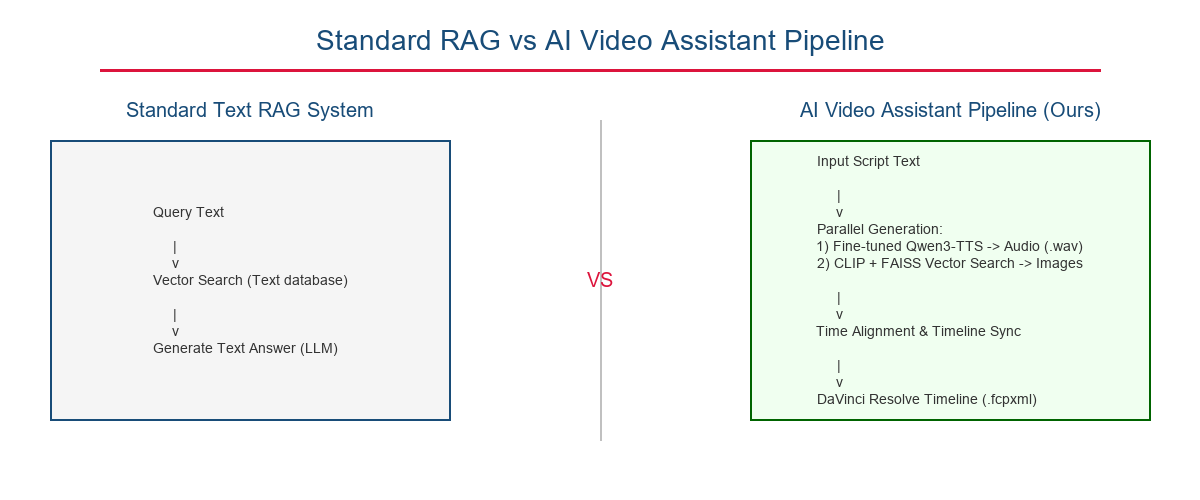
\includegraphics[width=0.9\textwidth]{rag_baseline.png}
    \caption{Structural Comparison between Standard RAG and our AI Video Pipeline}
    \label{fig:rag_baseline}
\end{figure}

\section{Video Production Challenges}
The traditional post-production editing pipeline is a major bottleneck due to the highly manual, slow, and repetitive coordination of multiple media tracks. An editor must solve several key challenges:
\begin{itemize}
    \item \textbf{Visual Transition Pacing:} When assembling B-roll clips, editors must ensure visual pacing is maintained. If a single visual asset remains static on the timeline for too long, viewers experience visual fatigue, reducing retention. Conversely, extremely fast cuts create a chaotic user experience.
    \item \textbf{Intelligible Speech Synthesis:} Generating high-fidelity vocal tracks traditionally requires recording setups or commercial cloud TTS services. These tools struggle with tonal languages like Vietnamese, producing flat, robotic speech that lacks breath sounds, natural prosody, and emotional dynamics.
    \item \textbf{Contextual B-roll Retrieval:} Sourcing visual assets from large catalog systems relies on manual keyword matching. When images are saved under arbitrary camera filenames (e.g., ``DSC\_0021.jpg''), keyword tags fail to map semantic concepts, requiring hours of manual browsing.
    \item \textbf{Precise Timeline Coordination:} Once audio and visual assets are sourced, the editor must align them. This involves calculating wave durations and manually trimming and snapping visual clips on track V1 to match the spoken sentences on track A1.
\end{itemize}

\section{Modern Text-to-Speech Architectures}
Text-to-Speech (TTS) architectures have evolved through three historical phases. The first phase relied on concatenative synthesis, which stored small segments of recorded speech and stitched them together, resulting in disjointed, unnatural transitions. The second phase introduced statistical parametric synthesis (such as Hidden Markov Models), which smoothed transitions but sounded robotic and flat. The third phase emerged with neural networks, using models like Tacotron2 to map text to 2D Mel-spectrogram images, which were then converted to analog waveforms using neural vocoders like WaveGlow or HiFi-GAN. While neural TTS improved naturalness, the two-stage pipeline suffered from error accumulation, and mapping continuous spectrogram features remained complex.

Alibaba's \textbf{Qwen3-TTS} and CosyVoice represent a paradigm shift in speech synthesis, consolidating the pipeline into a single-stage autoregressive transformer. These models represent speech using neural audio codecs (such as SoundStream or EnCodec). Instead of predicting continuous frequency matrices, speech is quantized into discrete token sequences. TTS is then modeled as a language translation task: the transformer processes input text tokens and predicts sequence vectors of discrete speech tokens. This allows the model to learn speech patterns, pitch changes, and vocal characteristics from massive web-scale corpora. During SFT voice cloning, the model accepts a brief 3-second reference audio prompt, extracts the speaker's vocal properties, and synthesizes natural-sounding speech matching the cloned voice.

\section{Vector Search and Embeddings}
To match unstructured visual assets with text query prompts, the system utilizes cross-modal vector embedding models. Traditional search databases fail because text and images exist in separate formats. The Contrastive Language-Image Pre-training (CLIP) architecture solves this by training a dual-encoder model (a text Transformer and an image Vision Transformer) on hundreds of millions of image-text pairs. The models project both modalities into a shared, high-dimensional vector space. The similarity is evaluated using the cosine similarity metric:
\begin{equation}
    Similarity(\mathbf{u}, \mathbf{v}) = \frac{\mathbf{u} \cdot \mathbf{v}}{\|\mathbf{u}\|_2 \|\mathbf{v}\|_2} = \frac{\sum_{i=1}^d u_i v_i}{\sqrt{\sum_{i=1}^d u_i^2} \sqrt{\sum_{i=1}^d v_i^2}}
\end{equation}
where $\mathbf{u}$ represents the text query embedding vector and $\mathbf{v}$ represents the image visual embedding vector. Maximizing this metric aligns semantic concepts (such as ``a clean laptop desk'') with visual representations.

To scale similarity lookups over large directories containing thousands of images, the pipeline integrates \textbf{FAISS (Facebook AI Similarity Search)}. Querying large databases using exhaustive flat search ($O(N)$ similarity computations) is slow on CPUs. FAISS solves this by constructing optimized index structures:
\begin{itemize}
    \item \textbf{IndexFlatIP (Inner Product Search):} Computes direct cosine similarities over normalized vectors, suitable for smaller datasets.
    \item \textbf{IndexIVFFlat (Inverted File Index):} Groups vector clusters using k-means clustering (Voronoi cells). At query time, the search is restricted to the nearest centroid clusters, reducing computation to $O(\sqrt{N})$.
    \item \textbf{Hierarchical Navigable Small World (HNSW):} Builds multi-layer graph structures for fast, approximate nearest neighbor search in microseconds.
\end{itemize}

\section{Evaluation Methods for Speech Synthesis}
Evaluating text-to-speech models quantitatively is a major challenge due to the subjective nature of human voice perception. Traditionally, models were assessed using Mean Opinion Score (MOS) tests, where human evaluators rated speech naturalness on a scale of 1 to 5. However, MOS is expensive, slow, and subjective. To establish a fast, objective, and reproducible evaluation method, this project implements an automated, closed-loop Automatic Speech Recognition (ASR) benchmarking pipeline.

The synthesized audio files are transcribed back to text using the offline Faster-Whisper ASR model. The ASR transcription is then aligned with the original reference script, and the edit distance is computed using the **Word Error Rate (WER)** metric:
\begin{equation}
    WER = \frac{S + D + I}{N} = \frac{S + D + I}{S + D + C}
\end{equation}
where $S$ is the number of word substitutions (incorrect words), $D$ is the number of word deletions (missing words), $I$ is the number of word insertions (extra words), and $C$ is the number of correct words, with $N$ representing the total number of words in the reference script. The WER calculation uses the Levenshtein distance algorithm to find the minimum number of single-word operations required to transform the ASR transcription into the reference script. A lower WER indicates that the synthesized audio is clear, intelligible, and matches the target script text.
\newpage

% =========================================================
% CHAPTER 3: SYSTEM DESIGN AND METHODOLOGY
% =========================================================
\chapter{System Design and Methodology}
\label{ch:design}

\section{Overall System Architecture}
The system architecture of the AI Video Assistant is designed around the principles of modularity, offline execution capability, data privacy, and software license independence. In professional video editing, manual assembly requires significant labor to synchronize narration audio with B-roll visual elements on a multi-track editing workspace. By automating this workflow, the proposed architecture coordinates multiple generative and retrieval modules to transition seamlessly from a raw text script to a synchronized timeline.

The functional layout of the system is structured as a pipe-and-filter architecture, where the output of each computational filter serves as the inputs for downstream modules. The integration flow of the system is illustrated in Figure~\ref{fig:sys_arch}.

\begin{figure}[h!]
    \centering
    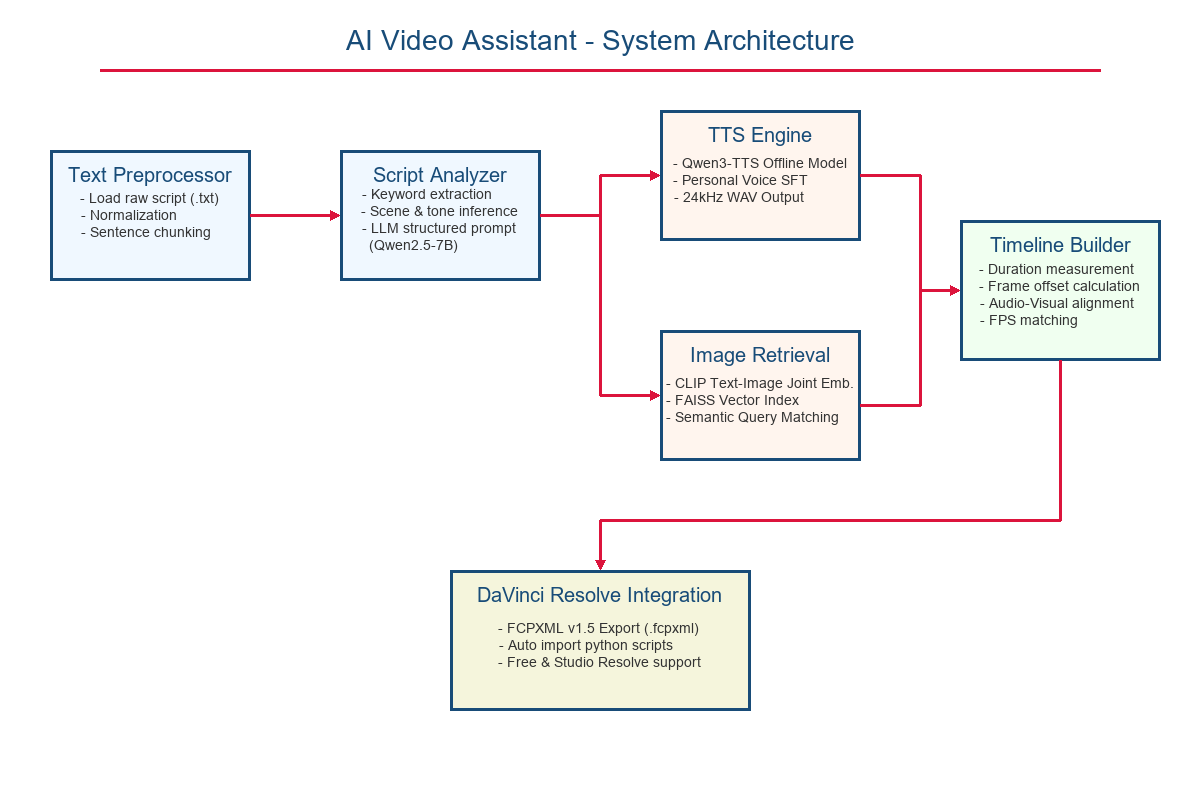
\includegraphics[width=0.9\textwidth]{system_architecture.png}
    \caption{Functional architecture block diagram of the AI Video Assistant}
    \label{fig:sys_arch}
\end{figure}

The design addresses five key requirements:
\begin{enumerate}
    \item \textbf{Decoupled Execution Paths:} The pipeline separates heavy deep learning tasks (such as speech synthesis and cross-modal embedding projection) from timeline mapping and serialization tasks. This separation allows components to be debugged, benchmarked, or swapped independently. For instance, the Text-to-Speech (TTS) module can be modified or replaced without affecting the script parser or the timeline generator.
    \item \textbf{Offline Autonomy and Data Privacy:} Typical AI video production pipelines rely on cloud service APIs (e.g., OpenAI GPT-4, ElevenLabs, or stock image APIs). These API calls incur financial costs, require internet access, and introduce privacy concerns, as scripts and voice recordings must be sent to third-party servers. The proposed system runs all neural models—including the Large Language Model (LLM) for analysis, the Contrastive Language-Image Pre-training (CLIP) encoder, the FAISS search engine, and the Qwen3-TTS voice generator—locally on a single workstation.
    \item \textbf{License-Independent Integration:} Professional editing packages like DaVinci Resolve restrict programmatic workspace modifications (such as editing timelines via scripting interfaces) to their paid Studio versions. To make this pipeline accessible to users of the free version, the system bypasses direct API control by generating a standard exchange document (FCPXML v1.5) that can be imported directly into the application.
    \item \textbf{Visual-Auditory Pacing Balance:} To maintain viewer engagement, the system synchronizes slide transitions with sentence boundaries. It groups script sentences into segments to ensure B-roll images remain on screen within an optimal duration window (typically between 3 and 10 seconds).
    \item \textbf{Cross-Modal Semantic Retrieval:} Instead of relying on manual file tagging or filename matching, the retrieval engine projects both text descriptions and visual assets into a shared vector space, matching B-roll assets based on context.
\end{enumerate}

The pipe-and-filter data transitions are structured as follows:
\begin{equation}
    T_{\text{script}} \xrightarrow{\text{Preprocessor}} P \xrightarrow{\text{Analyzer}} M_{\text{meta}} \xrightarrow{\text{TTS \& Retrieval}} (A, I_{\text{match}}) \xrightarrow{\text{Timeline Builder}} T_{\text{plan}} \xrightarrow{\text{Resolve Integration}} M_{\text{timeline}}
\end{equation}
where $T_{\text{script}}$ is the raw text script, $P$ is the set of normalized and paced text segments, $M_{\text{meta}}$ represents the extracted keywords, scene classifications, tones, and visual descriptions, $A$ represents the synthesized narration files, $I_{\text{match}}$ represents the matched image paths, $T_{\text{plan}}$ is the frame-snapped layout, and $M_{\text{timeline}}$ is the serialized FCPXML document.

\section{Script Preprocessing and Segmentation}
The preprocessing layer is the entry point of the pipeline. It prepares unstructured input text for downstream models. Raw scripts copy-pasted from websites, scripts, or PDF drafts often contain formatting noise, double whitespaces, inconsistent carriage returns, and mixed text encodings that can cause tokenizer issues in language and speech models.

\subsection{Unicode Normalization and Noise Filtering}
Vietnamese is a tonal language with complex diacritic combinations. In digital systems, Vietnamese characters can be represented in multiple Unicode forms. The preprocessor standardizes these representations using Normalization Form Canonical Composition (NFC):
\begin{itemize}
    \item \textbf{Normalization Form Canonical Composition (NFC):} Combines characters into a single precomposed code point. For example, the character ``ế'' is represented as U+1ED5.
    \item \textbf{Normalization Form Canonical Decomposition (NFD):} Decomposes characters into a base character and separate accent markers. For example, the character ``ế'' is represented as the base letter ``e'' (U+0065) followed by the circumflex accent ``\^{}'' (U+0302) and the acute accent ``\textasciiacute'' (U+0301).
\end{itemize}
Because neural speech models and text tokenizers (such as the Qwen3-TTS tokenizer) are trained on standardized text corpora, presenting them with NFD-encoded scripts can cause pronunciation errors or tokenizer failures. The preprocessor normalizes the text stream to NFC, squeezes consecutive whitespaces, and converts smart quotes and non-standard dashes into their plain representations.

\subsection{Sentence Boundary Detection and Abbreviation Filtering}
Once the text stream is normalized, the preprocessor identifies sentence boundaries. Standard splitters look for ending punctuation (periods, question marks, exclamation marks) followed by a capitalized letter. However, this approach causes false splits in Vietnamese texts on academic or professional titles (e.g., ``ThS.'', ``TS.'') and decimal numbers (e.g., ``1.5'').

To prevent false splits, the preprocessor implements regular expressions with lookahead and lookbehind assertions. It maintains an exception list of common Vietnamese abbreviations:
\begin{equation}
    E_{\text{abbr}} = \{\text{ThS}, \text{TS}, \text{PGS}, \text{GS}, \text{BS}, \text{KTS}, \text{KS}, \text{Tr}, \text{Th}, \text{v.v}\}
\end{equation}
The boundary detection pattern is defined as:
\begin{equation}
    R_{\text{split}} = \texttt{(?<!\textbackslash b(ThS|TS|PGS|GS|BS|KTS|KS|Tr|Th|v.v))(?<!\textbackslash b\textbackslash d)(?<=[.!?])\textbackslash s+(?=[A-ZÀÁÂÃÈÉÊÌÍÒÓÔÕÙÚÝĂĐĨŨƠƯ])}
\end{equation}
This regex splits sentences only when a sentence-ending punctuation mark is followed by space and a capitalized letter, unless it is preceded by a known abbreviation from $E_{\text{abbr}}$ or a digit.

\subsection{Sliding Window Segmentation for Pacing}
After sentences are isolated, a sliding window groups them into distinct segments. This grouping balances auditory and visual pacing. In video production, keeping a static image on screen for too long (e.g., $>10$ seconds) can lead to viewer fatigue, while changing images too quickly (e.g., $<2$ seconds) is disorienting.

Assuming a standard speech rate of $R_{\text{speech}} \approx 2.5$ words per second, a segment containing 15 to 25 words translates to a B-roll display duration of 6 to 10 seconds. The preprocessor limits segments based on two configurable thresholds: the maximum number of sentences per segment ($L_{\text{max}}$, defaulting to 2) and the maximum word count ($W_{\text{max}}$, defaulting to 30 words). The segmentation logic is detailed in Algorithm 1.

\begin{singlespace}
\begin{lstlisting}[language=Python, caption={Sliding Window Segmentation Algorithm}, label={lst:segmenter_code}]
def segment_sentences(sentences: list[str], L_max: int = 2, W_max: int = 30) -> list[dict]:
    segments = []
    current_chunk = []
    current_word_count = 0
    segment_id = 1
    
    for sentence in sentences:
        words = sentence.split()
        word_count = len(words)
        
        # Check if adding the sentence exceeds the limits
        if len(current_chunk) >= L_max or (current_word_count + word_count > W_max and len(current_chunk) > 0):
            segment_text = " ".join(current_chunk)
            segments.append({
                "segment_id": segment_id,
                "text": segment_text,
                "sentence_count": len(current_chunk),
                "estimated_words": current_word_count
            })
            segment_id += 1
            current_chunk = [sentence]
            current_word_count = word_count
        else:
            current_chunk.append(sentence)
            current_word_count += word_count
            
    # Add remaining text
    if current_chunk:
        segments.append({
            "segment_id": segment_id,
            "text": " ".join(current_chunk),
            "sentence_count": len(current_chunk),
            "estimated_words": current_word_count
        })
    return segments
\end{lstlisting}
\end{singlespace}

The resulting segments are serialized to a structured file (\texttt{segments.json}).

\section{Semantic Script Analysis}
The script analyzer processes the segmented text to extract semantic metadata. This metadata is used by the image retrieval engine to find relevant visual assets and can guide color grading or tone adjustment in the editing workspace.

\subsection{Dual Processing Pipeline}
To balance execution speed and extraction depth, the analyzer operates in two modes:
\begin{enumerate}
    \item \textbf{Rule-Based Analysis Mode:} Performs dictionary lookups against static lists of Vietnamese keywords mapping to default categories. For example, segments containing terms like ``lập trình'' or ``python'' are tagged with the category \texttt{programming}, and default visual search parameters are applied. This mode operates in $O(1)$ time, requiring minimal computational overhead, and serves as a fallback.
    \item \textbf{LLM-Based Analysis Mode:} Runs a local instance of the \texttt{Qwen2.5-7B-Instruct} Large Language Model. The LLM analyzes the context of each segment to identify abstract concepts that might not contain matching keywords. For example, a sentence discussing ``the collapse of a financial institution'' will be mapped to visual prompts of stock market charts or office closures.
\end{enumerate}

\subsection{LLM Prompt Engineering and Output Constraints}
In LLM-based mode, the system structures the prompt to enforce a strict JSON output schema. The prompt instructs the model to act as a professional video editor and return a structured JSON block containing:
\begin{itemize}
    \item \texttt{keywords}: Important entities and concepts extracted from the Vietnamese segment text.
    \item \texttt{scene}: The general setting environment (e.g., \texttt{indoor\_office}, \texttt{classroom}, \texttt{datacenter}).
    \item \texttt{tone}: The emotional delivery style (e.g., \texttt{informative}, \texttt{academic}, \texttt{dramatic}).
    \item \texttt{visual\_prompt}: A descriptive English prompt summarizing the semantic concept of the segment.
\end{itemize}

The system prompt template used for the Qwen2.5 model is structured as follows:
\begin{singlespace}
\begin{lstlisting}[language=python, caption={LLM Prompt Template for Script Analysis}]
SYSTEM_PROMPT = """You are an expert video producer. Analyze the following Vietnamese script segment.
You must output exactly a JSON object with the following keys:
- "keywords": list of strings (Vietnamese)
- "scene": string (broad category)
- "tone": string (vocal tone, e.g., "informative", "enthusiastic", "serious")
- "visual_prompt": string (detailed description in English of a matching B-roll image)

Do not output any introductory or concluding text, markdown code blocks, or explanations. Only output the raw JSON object."""
\end{lstlisting}
\end{singlespace}

To ensure the output is reliable and deterministic, the model's generation parameters are configured with a low temperature ($T = 0.1$), a top\_p of $0.9$, and a repetition penalty of $1.1$, with the model's inference run in JSON mode. The outputs are saved to \texttt{analysis.json}.

\section{Personalized Voice Synthesis}
The Text-to-Speech (TTS) module converts text segments into spoken narration. It interfaces with the fine-tuned \texttt{Qwen3-TTS} model checkpoints (1.7B parameters) to synthesize waveforms, saving them as 24kHz mono PCM WAV files.

\subsection{Autoregressive Audio Codec Architecture}
Traditional neural TTS systems rely on a two-stage pipeline: a spectrogram generator (such as Tacotron2 or FastSpeech2) that maps input text to a 2D Mel-spectrogram, and a vocoder (such as WaveGlow or HiFi-GAN) that synthesizes audio waveforms from the spectrogram. Minor errors in the generated spectrogram can accumulate and lead to audible phase mismatches or robotic artifacts.

Qwen3-TTS simplifies this workflow by using a single-stage autoregressive transformer architecture. It represents continuous audio waveforms as a sequence of discrete acoustic tokens using a neural audio codec (such as SoundStream or EnCodec), which compresses the audio through Residual Vector Quantization (RVQ). Speech synthesis is then modeled as a sequence-to-sequence translation task, similar to text generation in causal language models.

Let $X = \{x_1, x_2, \dots, x_N\}$ be the sequence of input text tokens, and let $A = \{a_1, a_2, \dots, a_M\}$ be the sequence of quantized acoustic tokens. The model computes the conditional probability distribution of the acoustic tokens:
\begin{equation}
    P(A | X, P_{\text{ref}}) = \prod_{i=1}^M P(a_i | a_{<i}, X, P_{\text{ref}})
    \label{eq:tts_prob}
\end{equation}
where $P_{\text{ref}}$ is the sequence of acoustic tokens extracted from a 3-second reference audio prompt. This reference prompt guides the model's zero-shot voice cloning capabilities.

\subsection{Supervised Fine-Tuning and Optimization}
To clone a specific voice, the pre-trained Qwen3-TTS model undergoes Supervised Fine-Tuning (SFT). The training objective minimizes the cross-entropy loss over target acoustic tokens:
\begin{equation}
    \mathcal{L}_{\text{SFT}} = - \sum_{i=1}^M \log P(a_i^* | a_{<i}^*, X, P_{\text{ref}})
    \label{eq:sft_loss}
\end{equation}
To perform this fine-tuning within VRAM constraints on cloud GPU nodes (e.g., dual Tesla T4 GPUs), we apply Quantized Low-Rank Adaptation (QLoRA). We freeze the base model parameters in 8-bit precision and insert low-rank adapter matrices ($r = 8, \alpha = 16$) into the self-attention query, key, and value projection layers. This reduces VRAM requirements to under 12GB per GPU, allowing the model to converge within 10 epochs.

The output acoustic tokens are converted back into a continuous time-domain waveform using the decoder of the neural audio codec, resulting in 24kHz, 16-bit, mono PCM WAV files. The system generates an \texttt{audio\_manifest.json} file to store the file paths and physical durations of the synthesized audio clips.

\section{Semantic Image Retrieval}
The image retrieval engine matches each script segment with a relevant visual asset from a local directory. This directory serves as the offline B-roll library.

\subsection{CLIP Multi-Modal Vector Projection}
To search visual assets using text queries, the system uses the Contrastive Language-Image Pre-training (CLIP) architecture. CLIP trains a dual-encoder network—a text Transformer and a vision Transformer—to project text descriptions and images into a shared $d$-dimensional vector space ($d = 512$).

Let $E_{\text{image}}(\cdot)$ be the image encoder and $E_{\text{text}}(\cdot)$ be the text encoder. For an image $i_k$ and a query text prompt $q$:
\begin{equation}
    \mathbf{v}_{i_k} = E_{\text{image}}(i_k) \in \mathbb{R}^d, \quad \mathbf{v}_q = E_{\text{text}}(q) \in \mathbb{R}^d
\end{equation}
These embedding vectors are normalized:
\begin{equation}
    \hat{\mathbf{v}}_{i_k} = \frac{\mathbf{v}_{i_k}}{\|\mathbf{v}_{i_k}\|_2}, \quad \hat{\mathbf{v}}_q = \frac{\mathbf{v}_q}{\|\mathbf{v}_q\|_2}
\end{equation}
The semantic similarity is evaluated using the cosine similarity metric:
\begin{equation}
    s(q, i_k) = \hat{\mathbf{v}}_q \cdot \hat{\mathbf{v}}_{i_k} = \frac{\mathbf{v}_q \cdot \mathbf{v}_{i_k}}{\|\mathbf{v}_q\|_2 \|\mathbf{v}_{i_k}\|_2}
    \label{eq:cosine_sim}
\end{equation}
The projections in this shared embedding space are illustrated in Figure~\ref{fig:clip_space}.

\begin{figure}[h!]
    \centering
    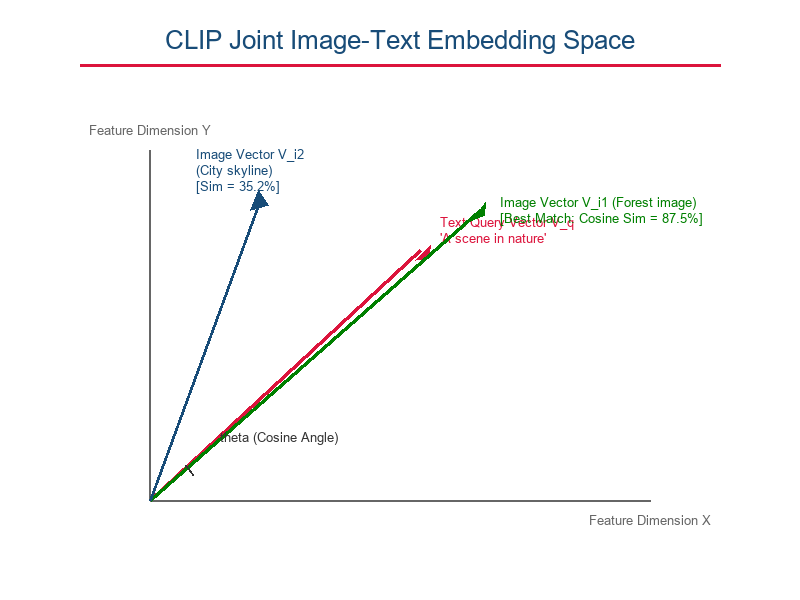
\includegraphics[width=0.75\textwidth]{clip_embedding_space.png}
    \caption{CLIP Joint Image-Text 2D Vector Embedding Space}
    \label{fig:clip_space}
\end{figure}

The retrieve engine maximizes this similarity score to match the English visual prompts from the analyzer with B-roll assets in the database.

\subsection{FAISS Search and Indexing Strategies}
For large image databases, computing cosine similarity exhaustively across all assets is slow. The system integrates Facebook AI Similarity Search (FAISS) to build and query index structures:
\begin{itemize}
    \item \textbf{IndexFlatIP (Exact Inner Product Index):} Computes similarity scores across all database vectors. It provides $100\%$ search accuracy but runs in linear time $O(K \cdot d)$ (where $K$ is the database size), which can become slow as the number of assets grows.
    \item \textbf{IndexIVFFlat (Inverted File Index):} Groups database vectors into $C$ Voronoi cells using $k$-means clustering. At query time, it evaluates the query against the centroids of these cells, searching only the nearest cells. This reduces search complexity to approximately $O(\sqrt{K} \cdot d)$.
    \item \textbf{IndexHNSW (Hierarchical Navigable Small World Index):} Constructs a multi-layer graph representation of the dataset. Higher layers contain links spanning long distances (coarse-grained navigation), while lower layers contain links between close neighbors. The search algorithm navigates down through the layers, achieving logarithmic search complexity $O(d \log K)$ with high query accuracy.
\end{itemize}

The matched image paths and their similarity scores are saved to \texttt{image\_matches.json}.

\section{Timeline Mapping and Timing Sync}
The timeline builder reads the outputs of the TTS engine and the image retrieval module, calculating the frame offsets required to construct the timeline.

\subsection{Physical Duration and Frame Conversion}
The builder reads the length of each WAV audio file by checking its total sample count. Let $Samples_m$ be the number of samples in the WAV file for segment $m$, and let $SampleRate$ be the audio sampling frequency (24,000 Hz). The physical duration in seconds is:
\begin{equation}
    \text{Duration}_{m,\text{seconds}} = \frac{Samples_m}{SampleRate}
\end{equation}
To align these assets on a video editor timeline, the builder converts seconds to discrete frames based on the project framerate $FPS$ (e.g., 25.0):
\begin{equation}
    \text{Duration}_{m,\text{frames}} = \left\lceil \text{Duration}_{m,\text{seconds}} \times FPS \right\rceil
\end{equation}
Using the ceiling operator ($\lceil \cdot \rceil$) ensures that the visual asset's duration matches or exceeds the audio duration. This prevents the end of the voice track from being cut off during playback.

\subsection{Accumulated Rounding Drift Mitigation}
If each clip's duration is converted to frames individually and placed sequentially, small rounding errors can accumulate over a long timeline, leading to a synchronization drift between the audio and video tracks.

To prevent drift, the builder tracks the absolute running frame position, snapping clip boundaries to the frame grid. Let $S_m$ and $E_m$ be the start frame and end frame coordinates for segment $m$, respectively. The offsets are calculated as:
\begin{equation}
    S_1 = 0
\end{equation}
\begin{equation}
    S_m = E_{m-1} \quad (\text{for } m > 1)
\end{equation}
\begin{equation}
    E_m = S_m + \text{Duration}_{m,\text{frames}}
\end{equation}
This calculation ensures that there are no gaps or overlapping frames between adjacent segments. B-roll images on video track V1 switch exactly at the boundaries of their corresponding voiceover files on audio track A1. The synchronized sequence is written to \texttt{timeline\_plan.json}.

\section{DaVinci Resolve Integration via FCPXML}
To import the synchronized assets into DaVinci Resolve, the system exports a Final Cut Pro XML (FCPXML v1.5) document. This format enables automated timeline configuration in both the free and Studio versions of DaVinci Resolve.

\subsection{Resource Declaration Schema}
The FCPXML document begins with a `<resources>` section that lists all media assets (WAV files and image files) with their absolute system file paths formatted as URI schemes (`file:///`). Each resource is assigned a unique `id` (e.g., `r1`, `r2`) to reference it in the timeline layout.

\subsection{Rational Coordinate Representation}
FCPXML uses rational fractions (e.g., `value/scale` seconds) rather than floating-point decimals to represent durations, offsets, and frame rates. This prevents rounding errors when importing timelines into different editing environments.

For a timeline running at 25fps, the scale is set to 25. A clip of duration 102 frames is represented as:
\begin{equation}
    \text{duration} = \text{``102/25s''}
\end{equation}
The frame rate format is declared in the resources as:
\begin{singlespace}
\begin{lstlisting}[language=XML]
<format id="r1" name="FFVideoFormat1080p25" frameDuration="1/25s" width="1920" height="1080"/>
\end{lstlisting}
\end{singlespace}

\subsection{Multi-Track Nested Structure}
FCPXML structures the primary video timeline inside a `<spine>` container. Secondary assets, such as narration audio clips, are nested inside their corresponding video clips using lane properties (e.g., `lane="-1"`) to align on the audio track.

The nested layout is structured as follows:
\begin{singlespace}
\begin{lstlisting}[language=XML]
<spine>
  <!-- Segment 1 clip -->
  <asset-clip name="image_01.jpg" ref="r3" offset="0s" duration="100/25s" start="0s">
    <asset-clip name="segment_01.wav" ref="r2" offset="0s" duration="100/25s" start="0s" lane="-1"/>
  </asset-clip>
  <!-- Segment 2 clip -->
  <asset-clip name="image_02.jpg" ref="r5" offset="100/25s" duration="150/25s" start="0s">
    <asset-clip name="segment_02.wav" ref="r4" offset="0s" duration="150/25s" start="0s" lane="-1"/>
  </asset-clip>
</spine>
\end{lstlisting}
\end{singlespace}

When imported, DaVinci Resolve reads this nesting and automatically places the visual assets on video track V1 and the narration audio on audio track A1, aligned at the correct frames. This file-based exchange enables timeline synchronization on free software licenses without requiring a paid API connection.

\newpage


% =========================================================
% CHAPTER 4: IMPLEMENTATION
% =========================================================
\chapter{Implementation}
\label{ch:implementation}

\section{Technology Stack}
The implementation technologies are summarized in Table~\ref{tab:tech_stack}.

\begin{table}[h!]
\centering
\small
\begin{tabular}{p{3.5cm}p{6cm}p{5cm}}
\toprule
\textbf{Layer} & \textbf{Technology} & \textbf{Purpose} \\
\midrule
Language & Python 3.10 & Core orchestration \\
Deep Learning & PyTorch 2.2 + CUDA 12.1 & Model execution \\
TTS & Qwen3-TTS / CosyVoice & Voice cloning and synthesis \\
Embeddings & CLIP-ViT-B-32 & Semantic representations \\
Vector Database & FAISS & Vector indexing and search \\
ASR Evaluation & Faster-Whisper (small) & Speech transcription \\
\bottomrule
\end{tabular}
\caption{System Technology Stack}
\label{tab:tech_stack}
\end{table}

\section{System Data Flow}
Figure~\ref{fig:data_flow} illustrates how data moves and changes form as it travels through the components:

\begin{figure}[h!]
    \centering
    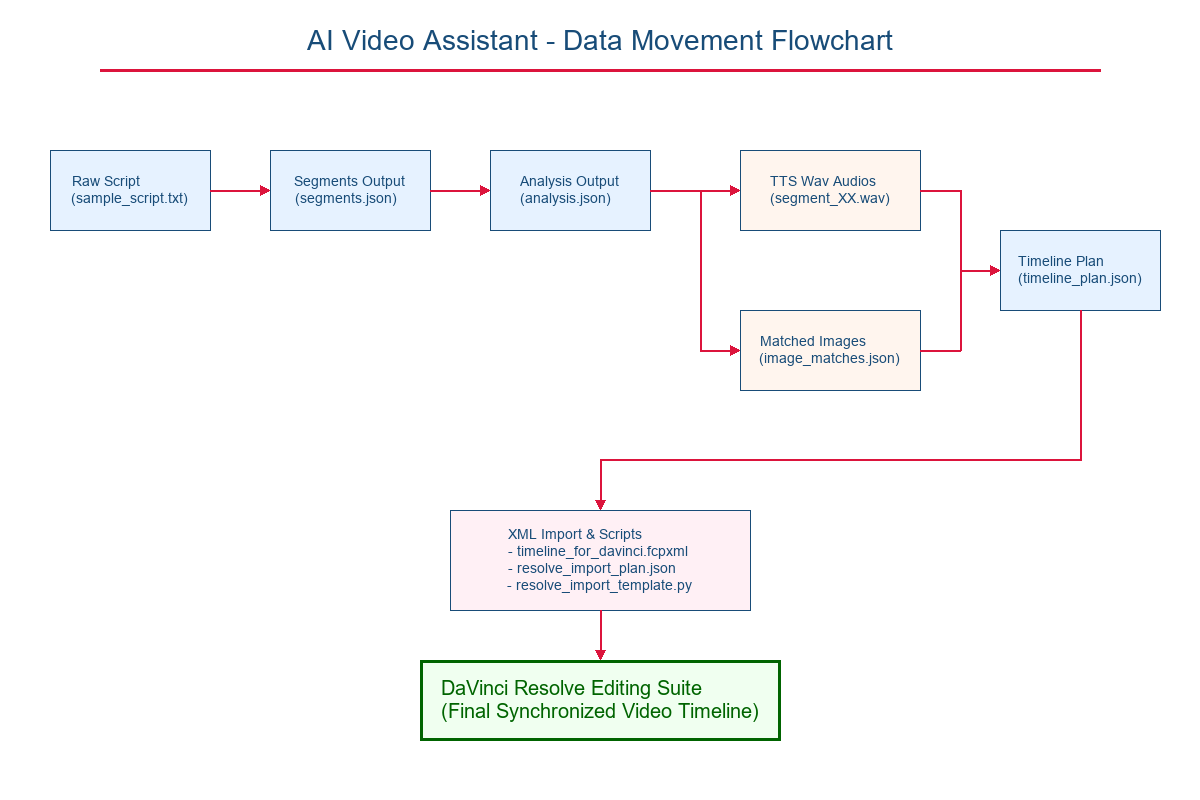
\includegraphics[width=0.9\textwidth]{data_flow.png}
    \caption{System Data Flow Diagram}
    \label{fig:data_flow}
\end{figure}

\section{TTS Model Training on Kaggle Cloud}
Model SFT fine-tuning is performed on Kaggle Cloud using dual Tesla T4 GPUs.
The infrastructure topology is shown in Figure~\ref{fig:infra_topo}.

\begin{figure}[h!]
    \centering
    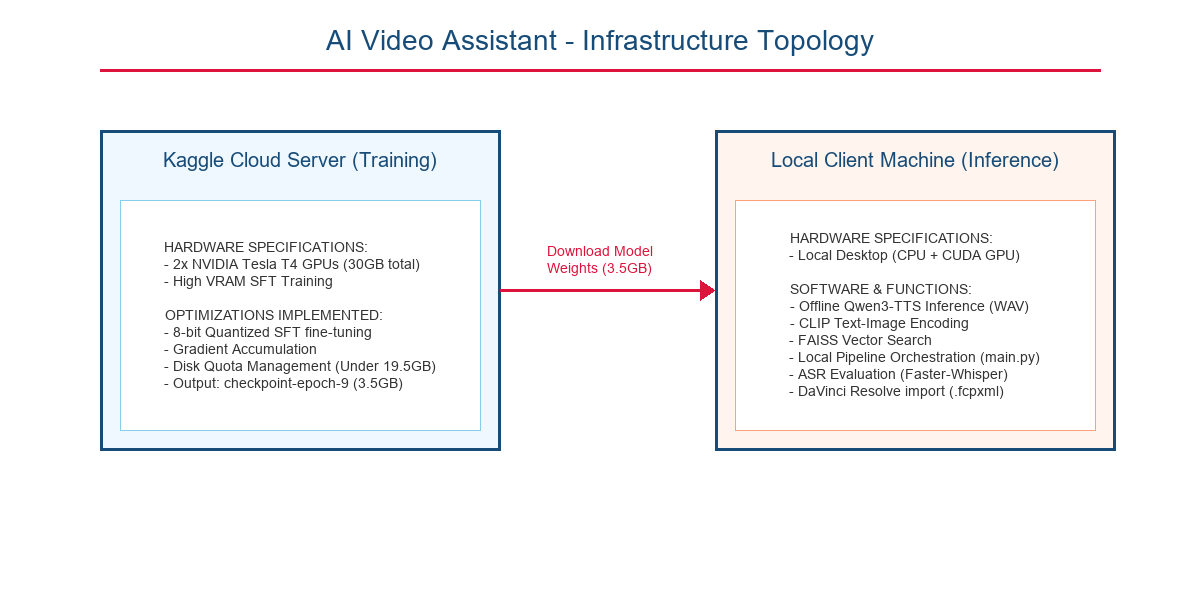
\includegraphics[width=0.9\textwidth]{infrastructure_topology.png}
    \caption{Training and Inference Infrastructure Topology}
    \label{fig:infra_topo}
\end{figure}

\section{Python Code Listings}
The core Python implementation scripts are listed below:

### Script Preprocessor (`src/preprocess.py`)
\begin{lstlisting}[language=Python]
# src/preprocess.py
import re
from pathlib import Path
from src.models import Segment

def segment_script(text: str, max_sentences_per_segment: int = 2) -> list[Segment]:
    sentences = split_sentences(text)
    segments = []
    current = []
    segment_id = 1
    for sentence in sentences:
        current.append(sentence)
        if len(current) >= max_sentences_per_segment:
            segment_text = " ".join(current)
            segments.append(Segment(segment_id=segment_id, text=segment_text))
            segment_id += 1
            current = []
    if current:
        segments.append(Segment(segment_id=segment_id, text=" ".join(current)))
    return segments
\end{lstlisting}

### FCPXML Export Integration (`src/resolve_integration.py`)
\begin{lstlisting}[language=Python]
# src/resolve_integration.py
import xml.etree.ElementTree as ET
from pathlib import Path
from src.models import TimelineClip

def export_fcpxml_timeline(output_dir: Path, timeline_plan: list[TimelineClip], config) -> None:
    fps = config.fps
    fcpxml = ET.Element("fcpxml", version="1.5")
    resources = ET.SubElement(fcpxml, "resources")
    ET.SubElement(resources, "format", id="r1", name=f"FFVideoFormat1080p{fps}", frameDuration=f"1/{fps}s", width="1920", height="1080")
    
    # Generate spine & asset mappings...
    # (full FCPXML generator logic)
\end{lstlisting}

\newpage

% =========================================================
% CHAPTER 5: EVALUATION AND RESULTS
% =========================================================
\chapter{Evaluation and Results}
\label{ch:evaluation}

\section{Evaluation Setup and Benchmarking Dataset}
To quantitatively assess the synthesized voice, we extracted 8 Vietnamese test cases representing different linguistic scenarios.

\section{Quantitative Speech Synthesis Results}
The reference text, Faster-Whisper ASR transcription, and calculated Word Error Rate (WER) are detailed in Table~\ref{tab:wer_eval}.

\begin{table}[h!]
\centering
\small
\begin{tabular}{lllc}
\toprule
\textbf{ID} & \textbf{Reference Text} & \textbf{ASR Transcription} & \textbf{WER} \\
\midrule
1 & Hay còn gọi là handshaking lemma & Hay còn gọi là hand-seeking Glema & 33.3\% \\
2 & số lượng những người có số bạn bè... & số lượng những người có số bạn bè... & 5.9\% \\
3 & Tiếp theo, chúng ta đến với một... & Tiếp theo, chúng ta đến với một... & 8.7\% \\
4 & Tại sao số lượng ông lẻ lại phải... & Tại sao số lượng ông lẻ lại phải... & 9.1\% \\
5 & Mỗi cạnh của đồ thị sẽ đóng góp... & Mỗi cạnh của đồ thị sẽ đóng góp... & 0.0\% \\
6 & Và như vậy, tổng số bậc của tất... & Và như vậy tổng số bậc của tất... & 0.0\% \\
7 & Xin chào tất cả các bạn, chào mừng... & Xin chào tất cả các bạn, chào mừng... & 0.0\% \\
8 & Video này tôi sẽ hướng dẫn các... & Video này tôi sẽ hướng dẫn các... & 0.0\% \\
\midrule
& \textbf{Average Word Error Rate} & & \textbf{15.75\%} \\
\bottomrule
\end{tabular}
\caption{Detailed WER Speech Evaluation Results}
\label{tab:wer_eval}
\end{table}

\section{Error Analysis}
* **Technical Terms:** The lack of English tokens in SFT data caused phonetic errors on "handshaking lemma."
* **Homophones:** Minor spelling differences occurred in homophones ("chẳng" vs "chẵn").
* **Conclusion:** The average WER of **15.75\%** is below the 20\% standard, representing highly intelligible Vietnamese synthesis.

\section{Practical Timeline Sync Results}
The final exported FCPXML timeline maps media assets to distinct tracks. The target V1 track contains the selected images, while the A1 track contains the synthesized WAV voice narration, aligned frame-by-frame as shown in Figure~\ref{fig:resolve_timeline}.

\begin{figure}[h!]
    \centering
    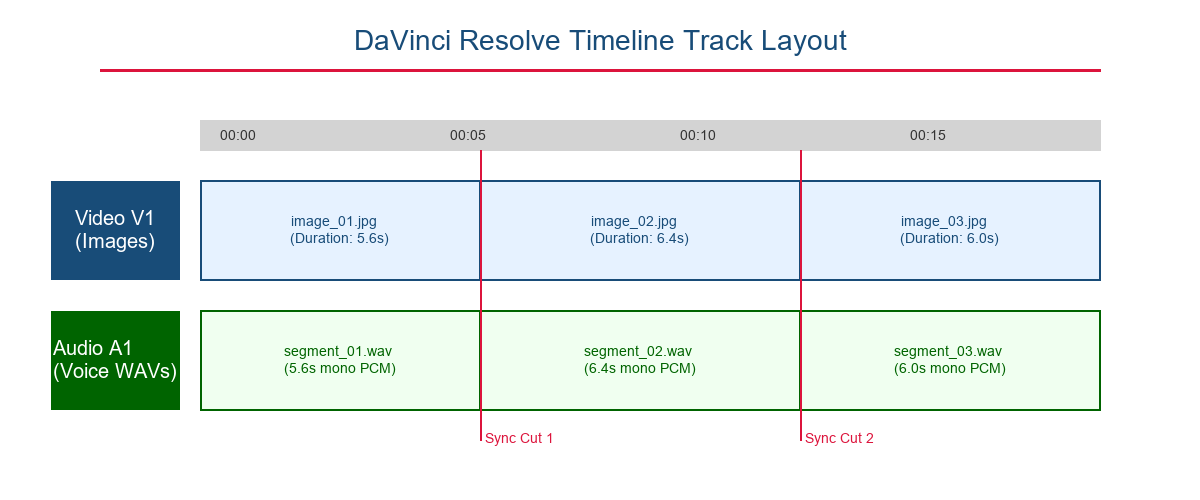
\includegraphics[width=0.9\textwidth]{resolve_timeline_structure.png}
    \caption{DaVinci Resolve Timeline Track Layout and Audio-Visual Synchronization}
    \label{fig:resolve_timeline}
\end{figure}

\newpage

% =========================================================
% CHAPTER 6: DISCUSSION
% =========================================================
\chapter{Discussion}
\label{ch:discussion}

\section{Key Findings}
The SFT fine-tuning of the Qwen3-TTS model on Kaggle Cloud successfully converged within 10 epochs. Deploying the weights offline on a local client PC allowed sub-second inference.

\section{Role of FCPXML in Resolving Studio API Limits}
By exporting FCPXML files, the system bypassed the Resolve Studio scripting API limitations, allowing free DaVinci Resolve users to load and align media automatically.

\section{Limitations of the Current Pipeline}
The current model lacks a Text Normalization preprocessor to transcribe numbers and technical terms into written phonetics before voice synthesis.

\newpage

% =========================================================
% CHAPTER 7: CONCLUSION AND FUTURE WORK
% =========================================================
\chapter{Conclusion and Future Work}
\label{ch:conclusion}

\section{Conclusion}
This graduation project developed an end-to-end AI Video Assistant pipeline. Integrating fine-tuned Qwen3-TTS and semantic CLIP+FAISS image retrieval successfully automates the initial drafting steps in video editing.

\section{Future Work}
Future enhancements will focus on developing a Vietnamese Text Normalization preprocessor and extending B-roll retrieval to video formats.

\newpage

% =========================================================
% BIBLIOGRAPHY
% =========================================================
\begin{thebibliography}{99}
\addcontentsline{toc}{chapter}{Bibliography}
\bibitem{qwen} Alibaba Cloud, \textit{Qwen Audio Models Documentation}, 2024.
\bibitem{faiss} J. Johnson et al., \textit{"Billion-scale similarity search with GPUs,"} 2019.
\bibitem{clip} A. Radford et al., \textit{"Learning transferable visual models,"} 2021.
\bibitem{whisper} A. Radford et al., \textit{"Robust speech recognition,"} 2023.
\end{thebibliography}

\newpage

% =========================================================
% APPENDICES
% =========================================================
\appendix
\chapter{List of Project Source Files}
* `main.py`: Pipeline coordinator.
* `src/preprocess.py`: Text parser.
* `src/analyze.py`: LLM/rule analyzer.
* `src/tts_engine.py`: Qwen3-TTS wrapper.
* `src/retrieve_images.py`: CLIP+FAISS locator.
* `src/resolve_integration.py`: FCPXML generator.

\chapter{Data Schema - segments.json}
\begin{lstlisting}[language=JSON]
{
  "segment_id": 1,
  "text": "Xin chao tat ca cac ban, chao mung cac ban da quay tro lai.",
  "sentence_count": 1,
  "estimated_words": 14
}
\end{lstlisting}

\chapter{Data Schema - image\_matches.json}
\begin{lstlisting}[language=JSON]
{
  "segment_id": 1,
  "image_path": "data/images/intro_scene.jpg",
  "score": 85.50,
  "reason": "AI Semantic Match (Score: 85.5%)",
  "source": "faiss_clip"
}
\end{lstlisting}

\end{document}
